\documentclass[12pt,letterpaper,final]{article}
\usepackage[utf8]{inputenc}
\usepackage{amsmath}
\usepackage{amsfonts}
\usepackage{amssymb}
\usepackage{graphicx}
\graphicspath{{images/}}
\usepackage{cite}
\usepackage{enumerate}
\usepackage{url}
\usepackage{listings}
\usepackage[UKenglish]{babel}% http://ctan.org/pkg/babel
\usepackage{booktabs}
\usepackage[table,xcdraw]{xcolor}
\usepackage[T1]{fontenc}
\usepackage[scaled]{helvet}
\renewcommand*\familydefault{\sfdefault}
\usepackage{hyperref}
\hypersetup{
    colorlinks=true,
    linkcolor=blue,
    filecolor=magenta,      
    urlcolor=cyan,
}
 
\urlstyle{same}


\title{Light and Electron microscopes comparison}
\date{\today} 
\author{Max Sepulveda}

\begin{document}
\maketitle

A microscope is an instrument that magnifies objects otherwise too small to be seen, producing an image in which the object appears larger. Most photographs of cells are taken using a microscope, and these pictures can also be called \emph{micrographs}.

From the definition above, it might sound like a microscope is just a kind of magnifying glass. In fact, magnifying glasses do qualify as microscopes; since they have just one lens, they are called simple microscopes. The fancier instruments that we typically think of as microscopes are compound microscopes, meaning that they have multiple lenses. 

Because of the way these lenses are arranged, they can bend light to produce a much more magnified image than that of a magnifying glass.

In a compound microscope with two lenses, the arrangement of the lenses has an interesting consequence: the orientation of the image you see is flipped in relation to the actual object you’re examining. For example, if you were looking at a piece of newsprint with the letter ``A'' on it, the image you saw through the microscope would be ``$\forall$''. 

More complex compound microscopes may not produce an inverted image because they include an additional lens that “re-inverts” the image back to its normal state.
 
\bigskip

The following table \ref{tab:my-table} presents a comparison of the main characteristics for both a light microscope and an electron microscope.


\begin{table}[]
\centering
\LARGE
\resizebox{\columnwidth}{!}{%
\begin{tabular}{@{}|l|l|@{}}
\toprule
\rowcolor[HTML]{C0C0C0} 
\multicolumn{1}{|c|}{\LARGE \cellcolor[HTML]{C0C0C0}{\color[HTML]{333333} Light Microscope }} & \multicolumn{1}{c|}{\LARGE \cellcolor[HTML]{C0C0C0} Electron Microscope}  \\ \midrule
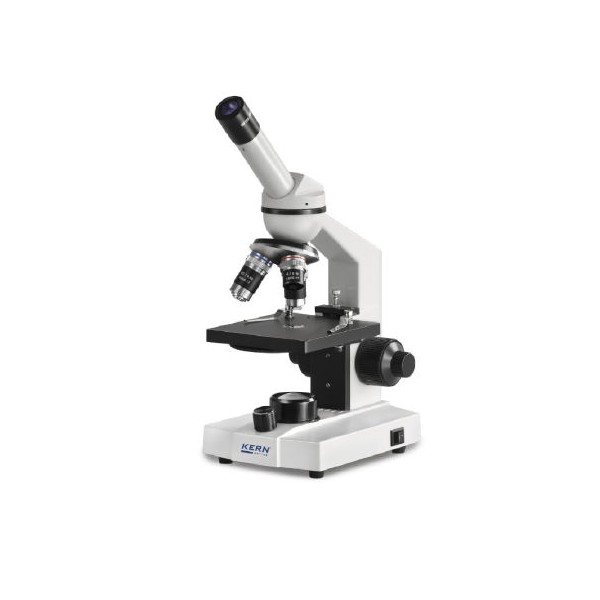
\includegraphics[width=6in]{light} &  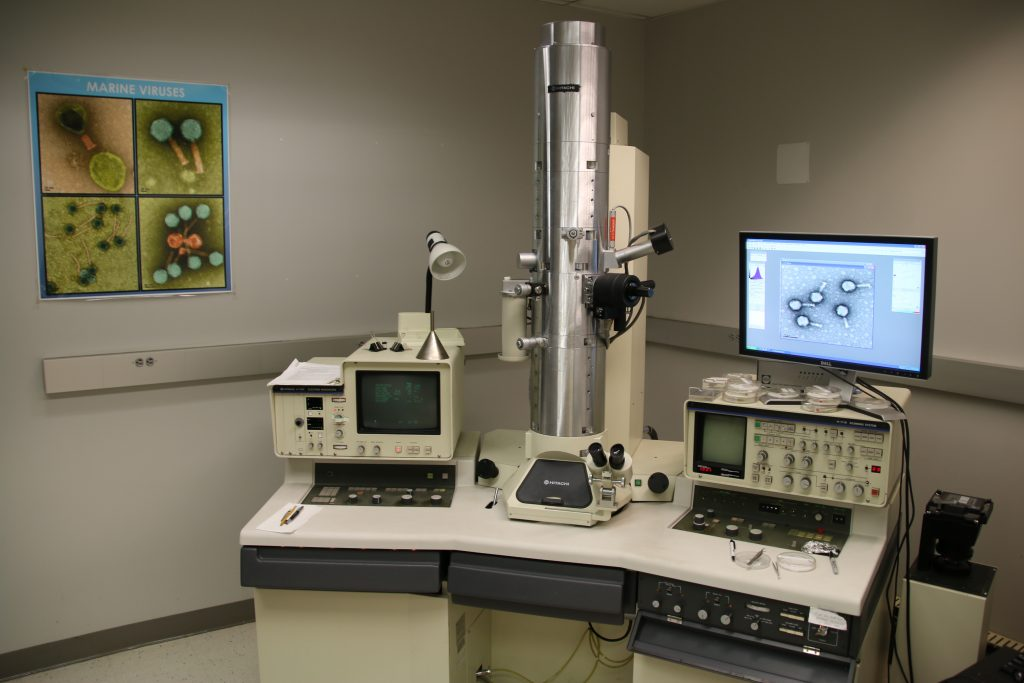
\includegraphics[width=6in]{electron} \\ \midrule

\LARGE Use light to provide magnification & \LARGE Use beams of electrons to work \\ \midrule
\LARGE Image is coloured &  \LARGE Image is in black and white \\ \midrule
\LARGE Controls image formation via glass lenses &  \LARGE Beams of electrons can be focused using electromagnets \\ \midrule
\LARGE No radiation risk &  \LARGE Risk of radiation leakage \\ \bottomrule
\LARGE \textbf{Magnification} from 500x to 1500x &  \LARGE Magnification of 100000x to 300000x \\ \bottomrule
\LARGE The \textbf{specimen} can be dead or alive &  \LARGE Specimen must be dead or dried \\ \bottomrule
\LARGE It is used for the study of detailed gross internal structure  &  \LARGE Used for external surface, ultra structure of cell \\ \bottomrule
\LARGE No \textbf{filament} is used &  \LARGE A tungsten filament is used to produce electrons \\ \bottomrule  
\end{tabular}%
}
\caption{Microscopes comparison}
\label{tab:my-table}
\end{table}

\newpage

\textbf{Glossary}
\begin{itemize}

\item Filament: A conducting wire or thread with a high melting point, forming part of an electric bulb or thermionic valve and heated or made incandescent by an electric current.    

\item Specimen: An individual animal, plant, piece of a mineral, etc. used as an example of its species or type for scientific study or display.

\item Magnification: Enlarging the size of an object in an image so you can observe in greater detail

\end{itemize}


\begin{thebibliography}{9}
 
\bibitem{microscopy} 
Khan Academy, Microscopy.
\href{https://www.khanacademy.org/science/high-school-biology/hs-cells/hs-introduction-to-cells/a/microscopy}{https://www.khanacademy.org/science/high-school-biology/hs-cells/hs-introduction-to-cells/a/microscopy}
 
\bibitem{info} 
Microbiology Info, Differences between Light Microscope and Electron Microscope.
\href{https://microbiologyinfo.com/differences-between-light-microscope-and-electron-microscope/}{https://microbiologyinfo.com/differences-between-light-microscope-and-electron-microscope} 

\end{thebibliography}


\end{document}
